
\documentclass[12pt]{article} 
\usepackage[brazil]{babel} %hifenização em português do brasil
\usepackage{gensymb}
\usepackage[pdftex]{hyperref}
\usepackage[T1]{fontenc} % caracteres com acentos são considerados um bloco só
\usepackage{graphicx}
\usepackage{ae} %arruma a fonte quando usa o pacote acima
\usepackage[utf8]{inputenc}
\usepackage{graphicx}%Para inserir figuras

\usepackage{cite}

\begin{document} % Aqui começa o documento
\title{Implementação system calls no kernel linux V. 4.13.12\vspace{3.5cm}} % título

\author{
	João Paulo de Oliveira
	\texttt{joaopaulodeoliveira123@gmail.com}
	\and
	Lucas Rossi Rabelo
	\texttt{lucasrossi98@hotmail.com}
	\and		
	Matheus Pimenta Reis
	\texttt{}
	\vspace*{9cm}
}

\maketitle
\tableofcontents

\pagebreak
\section*{Implementação System Calls no Linux}
As System Calls fazer o interfaceamento entre o hardware e os processo do espaço de usuário, elas também servem para três propósitos principais:
\begin{enumerate}
	\item Provém abstração com o hardware para que o usuário tenha um maior rendimento. Por exemplo, o usuário não se preocupa com o tipo de partição em que ele lerá um arquivo;
	\item As system calls garantem a segurança e estabilidade para que um usuário relativamente leigo possa ter um alto rendimento com gerência de permissão, usuários e outros critérios de gerência do kernel;
	\item Uma camada entre espaço de usuário e o resto do sistema permite fornece o sistema virtualizado para os processos.
\end{enumerate}
	As chamadas syscalls em linux são, na maioria dos casos, acessadas pelas funções definidas na C library. As syscalls em si retornam um valor do tipo long4 que, quando negativo, em geral, denota um erro, já o retorno com valor zero (nem sempre) é um sinal de sucesso. A C library, quando uma system call retorna um erro, ela grava o código desse erro na variável global errno, que pode ser ser traduzida para um texto que fala sobre o erro através de funções de biblioteca.
	
	Para a implementação de uma system call deve-se ter acesso ao código do kernel do sistema operacional para tanto, foi escolhido o kernel Linux que é open source.
\subsection*{Download do Kernel}
Por ser open source, o código fonte do kernel do Linux é mantido online para livre acesso no GitHub(\url{https://github.com/torvalds/linux}), e também em The Linux Kernel Archives (\url{https://www.kernel.org/}) em várias versões e formatos de arquivos(compactados). A versão mais recente dado a data de início do TCD foi a versão \textbf{14.13.12}.
de gerência do kernel.
	A Free Software Foundation mantém, gerencia e presta suporte para o The Linux Kernel Archives.O donwnload do kernel pode ser feito facilmente, além de outras funções com perguntas frequentes, download de versões em teste (beta) para ser compilado em qualquer distribuição linux ou em outras plataformas que suportam o kernel.
	\vspace*{2cm}
	 Como pode ser visto na imagem abaixo:
\begin{figure}[!h]
	\centering
	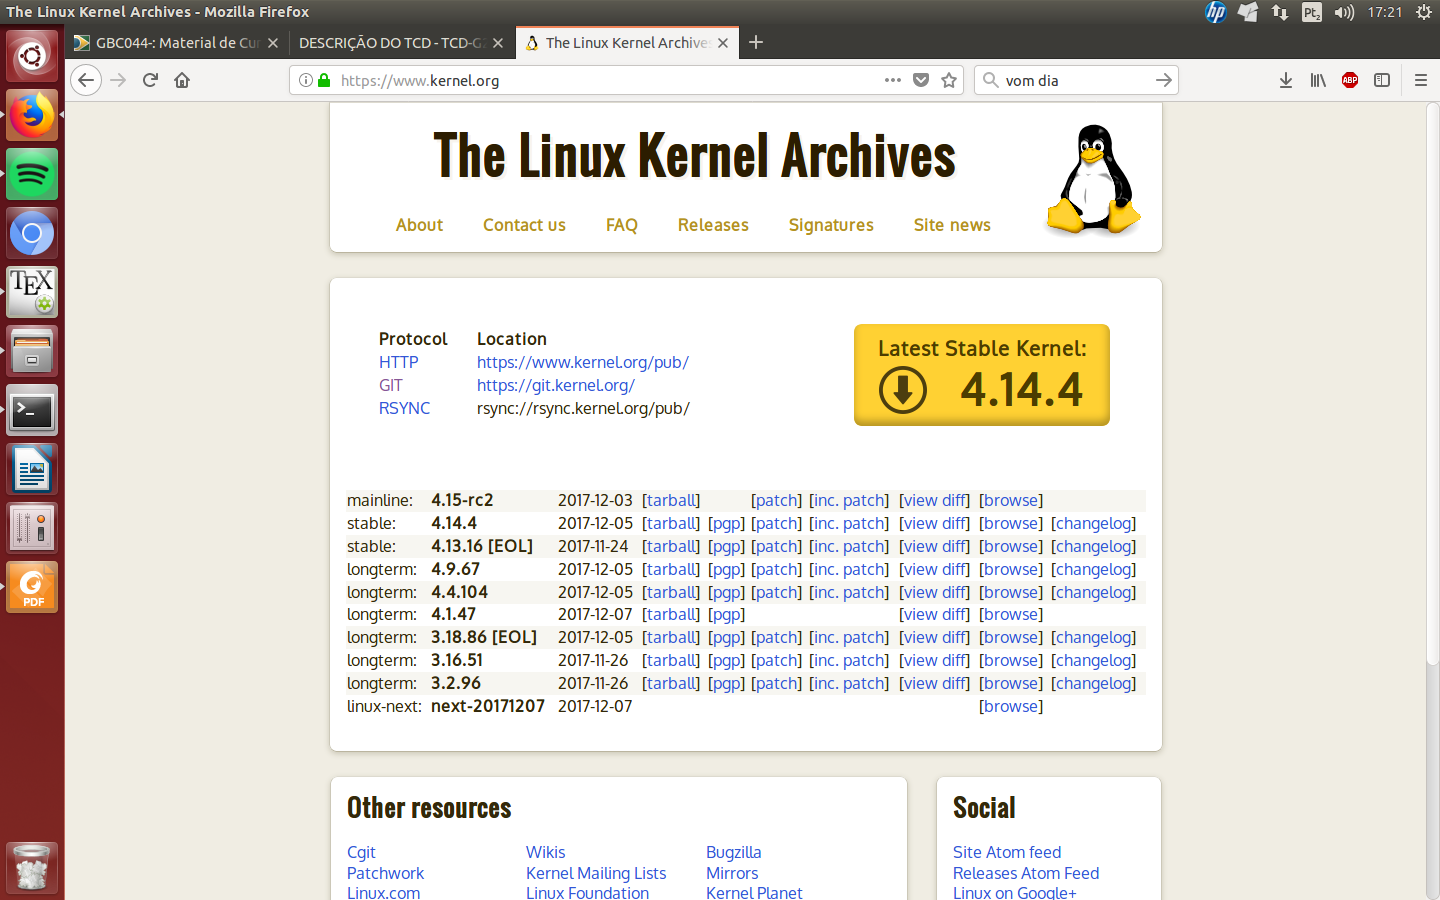
\includegraphics[scale=0.2]{imagens/kernelorg.png}
	\caption{The Linux Kernel Archives: Local de download do Kernel}
	\label{kernelorg}
\end{figure}
\subsection*{Criação da System Call}
\subsubsection*{Tempo na CPU}
\subsubsection*{Tempo de vida do processo}
\subsubsection*{N$^{\circ}$  de vezes que o processo passou pela CPU}
\subsection*{Código da system call}
\subsection*{Compilação do kernel}
\subsection*{Programa usuário da system call}




\bibliographystyle{abbrv}
\bibliography{refs}
\end{document}
